% \def\bmode{0} % Mode 0 for presentation, mode 1 for a handout with notes, mode 2 for handout without notes
% \if 0\bmode
% \documentclass[smaller]{beamer}
% \else \if 1\bmode
% \immediate\write18{pdflatex -jobname=\jobname-Notes-Handout\space\jobname}
\documentclass[smaller]{beamer}
%\usepackage{handoutWithNotes}
%\pgfpagesuselayout{2 on 1 with notes}[letterpaper, landscape, border shrink=4mm]
% \else \if 2\bmode
% \immediate\write18{pdflatex -jobname=\jobname_Handout\space\jobname}
% \documentclass[smaller,handout]{beamer}
% \fi
% \fi
% \fi


% \documentclass[smaller,handout
% ]{beamer}
%\usepackage{etex}
%\newcommand{\num}{6{} }

% \usetheme[
%   outer/progressbar=foot,
%   outer/numbering=counter,
%  block=fillFF
% ]{metropolis}

%\useoutertheme{metropolis}

\usetheme{Madrid}
\useoutertheme[subsection=false]{miniframes} % Alternatively: miniframes, infolines, split
\useinnertheme{circles}
\usecolortheme{seahorse}

\usepackage[backend=biber,style=authoryear,maxcitenames=2,maxbibnames=99,safeinputenc,url=false,
eprint=false]{biblatex}
\addbibresource{bib/references.bib}
\AtEveryCitekey{\iffootnote{{\tiny}\tiny}{\tiny}}
\usepackage{appendixnumberbeamer}
%\usepackage{pgfpages}
%\setbeameroption{hide notes} % Only slides
%\setbeameroption{show only notes} % Only notes
%\setbeameroption{hide notes} % Only notes
%\setbeameroption{show notes on second screen=right} % Both

% \usepackage[sfdefault]{Fira Sans}

% \setsansfont[BoldFont={Fira Sans}]{Fira Sans Light}
% \setmonofont{Fira Mono}

%\usepackage{fira}
%\setsansfont{Fira}
%\setmonofont{Fira Mono}
% To give a presentation with the Skim reader (http://skim-app.sourceforge.net) on OSX so
% that you see the notes on your laptop and the slides on the projector, do the following:
% 
% 1. Generate just the presentation (hide notes) and save to slides.pdf
% 2. Generate onlt the notes (show only nodes) and save to notes.pdf
% 3. With Skim open both slides.pdf and notes.pdf
% 4. Click on slides.pdf to bring it to front.
% 5. In Skim, under "View -> Presentation Option -> Synhcronized Noted Document"
%    select notes.pdf.
% 6. Now as you move around in slides.pdf the notes.pdf file will follow you.
% 7. Arrange windows so that notes.pdf is in full screen mode on your laptop
%    and slides.pdf is in presentation mode on the projector.

% Give a slight yellow tint to the notes page
%\setbeamertemplate{note page}{\pagecolor{yellow!5}\insertnote}\usepackage{palatino}


%\usetheme{metropolis}
%\usecolortheme{beaver}
\usepackage{xcolor}
\definecolor{darkcandyapplered}{HTML}{A40000}
\definecolor{lightcandyapplered}{HTML}{e74c3c}

%\setbeamercolor{title}{fg=darkcandyapplered}
%\setbeamercolor{frametitle}{bg=darkcandyapplered!80!black!90!white}
%\setbeamertemplate{frametitle}{\bf\insertframetitle}
%\setbeamercolor{footnote mark}{fg=darkcandyapplered}
%\setbeamercolor{footnote}{fg=darkcandyapplered!70}
%\Raggedbottom
%\setbeamerfont{page number in head/foot}{size=\tiny}
%\usepackage[tracking]{microtype}


\setbeamertemplate{frametitle}{%
    \nointerlineskip%
    \begin{beamercolorbox}[wd=\paperwidth,ht=2.0ex,dp=0.6ex]{frametitle}
        \hspace*{1ex}\insertframetitle%
    \end{beamercolorbox}%
}



\setbeamerfont{caption}{size=\footnotesize}
\setbeamercolor{caption name}{fg=darkcandyapplered}


%\usepackage[sc,osf]{mathpazo}   % With old-style figures and real smallcaps.
%\linespread{1.025}              % Palatino leads a little more leading

% Euler for math and numbers
%\usepackage[euler-digits,small]{eulervm}
%\AtBeginDocument{\renewcommand{\hbar}{\hslash}}
\usepackage{graphicx,multirow,paralist,booktabs}


%\mode<presentation> { \setbeamercovered{transparent} }

\setbeamertemplate{navigation symbols}{}
\makeatletter
\def\beamerorig@set@color{%
  \pdfliteral{\current@color}%
  \aftergroup\reset@color
}
\def\beamerorig@reset@color{\pdfliteral{\current@color}}
\makeatother

%=== GRAPHICS PATH ===========
\graphicspath{{./images/}}
% Marginpar width
%Marginpar width
%\setlength{\marginparsep}{.02in}


%% Captions
% \usepackage{caption}
% \captionsetup{
%   labelsep=quad,
%   justification=raggedright,
%   labelfont=sc
% }

%AMS-TeX packages

\usepackage{amssymb,amsmath,amsthm} 
\usepackage{bm}
\usepackage{color}

\usepackage{hyperref,enumerate}
\usepackage{minitoc,array}


%https://tex.stackexchange.com/a/31370/2269
\usepackage{mathtools,cancel}

\renewcommand{\CancelColor}{\color{red}} %change cancel color to red

\makeatletter
\let\my@cancelto\cancelto %copy over the original cancelto command
\newcommand<>{\cancelto}[2]{\alt#3{\my@cancelto{#1}{#2}}{\mathrlap{#2}\phantom{\my@cancelto{#1}{#2}}}}
% redefine the cancelto command, using \phantom to assure that the
% result doesn't wiggle up and down with and without the arrow
\makeatother


\definecolor{slblue}{rgb}{0,.3,.62}
\hypersetup{
    colorlinks,%
    citecolor=blue,%
    filecolor=blue,%
    linkcolor=blue,
    urlcolor=slblue
}

%%% TIKZ
\usepackage{animate}
\usepackage{tikz}
\usepackage{pgfplots}
\usepackage{pgfplotstable}
\usepackage{pgfgantt}
\usepackage{tikzsymbols}
\pgfplotsset{compat=newest}
\usepgfplotslibrary{groupplots,fillbetween}

\usetikzlibrary{arrows,shapes,positioning,shapes.geometric}
\usetikzlibrary{decorations.markings}
\usetikzlibrary{shadows,automata}
\usetikzlibrary{patterns,matrix}
\usetikzlibrary{trees,mindmap,backgrounds}
%\usetikzlibrary{circuits.ee.IEC}
\usetikzlibrary{decorations.text}
% For Sagnac Picture
\usetikzlibrary{%
    decorations.pathreplacing,%
    decorations.pathmorphing%
}
\tikzset{no shadows/.style={general shadow/.style=}}
%
%\usepackage{paralist}



%%% FORMAT PYTHON CODE
%\usepackage{listings}
% Default fixed font does not support bold face
\DeclareFixedFont{\ttb}{T1}{txtt}{bx}{n}{8} % for bold
\DeclareFixedFont{\ttm}{T1}{txtt}{m}{n}{8}  % for normal

% Custom colors
\definecolor{deepblue}{rgb}{0,0,0.5}
\definecolor{deepred}{rgb}{0.6,0,0}
\definecolor{deepgreen}{rgb}{0,0.5,0}
 

%\usepackage{listings}

% Python style for highlighting
% \newcommand\pythonstyle{\lstset{
% language=Python,
% basicstyle=\footnotesize\ttm,
% otherkeywords={self},             % Add keywords here
% keywordstyle=\footnotesize\ttb\color{deepblue},
% emph={MyClass,__init__},          % Custom highlighting
% emphstyle=\footnotesize\ttb\color{deepred},    % Custom highlighting style
% stringstyle=\color{deepgreen},
% frame=tb,                         % Any extra options here
    % showstringspaces=false            % 
% }}

% % Python environment
% \lstnewenvironment{python}[1][]
% {
% \pythonstyle
% \lstset{#1}
% }
% {}

% % Python for external files
% \newcommand\pythonexternal[2][]{{
% \pythonstyle
% \lstinputlisting[#1]{#2}}}

% Python for inline
% 
% \newcommand\pythoninline[1]{{\pythonstyle\lstinline!#1!}}


\newcommand{\osn}{\oldstylenums}
\newcommand{\dg}{^{\circ}}
\newcommand{\lt}{\left}
\newcommand{\rt}{\right}
\newcommand{\pt}{\phantom}
\newcommand{\tf}{\therefore}
\newcommand{\?}{\stackrel{?}{=}}
\newcommand{\fr}{\frac}
\newcommand{\dfr}{\dfrac}
\newcommand{\ul}{\underline}
\newcommand{\tn}{\tabularnewline}
\newcommand{\nl}{\newline}
\newcommand\relph[1]{\mathrel{\phantom{#1}}}
\newcommand{\cm}{\checkmark}
\newcommand{\ol}{\overline}
\newcommand{\rd}{\color{red}}
\newcommand{\bl}{\color{blue}}
\newcommand{\pl}{\color{purple}}
\newcommand{\og}{\color{orange!90!black}}
\newcommand{\gr}{\color{green!40!black}}
\newcommand{\nin}{\noindent}
\newcommand{\la}{\lambda}
\renewcommand{\th}{\theta}
\newcommand{\al}{\alpha}
\newcommand{\G}{\Gamma}
\newcommand*\circled[1]{\tikz[baseline=(char.base)]{
            \node[shape=circle,draw,thick,inner sep=1pt] (char) {\small #1};}}

\newcommand{\bc}{\begin{compactenum}[\quad--]}
\newcommand{\ec}{\end{compactenum}}

\newcommand{\p}{\partial}
\newcommand{\pd}[2]{\frac{\partial{#1}}{\partial{#2}}}
\newcommand{\dpd}[2]{\dfrac{\partial{#1}}{\partial{#2}}}
\newcommand{\pdd}[2]{\frac{\partial^2{#1}}{\partial{#2}^2}}
\newcommand{\nmfr}[3]{\Phi\left(\frac{{#1} - {#2}}{#3}\right)}


\pgfmathdeclarefunction{poiss}{1}{%
  \pgfmathparse{(#1^x)*exp(-#1)/(x!)}%
  }

\pgfmathdeclarefunction{gauss}{2}{%
  \pgfmathparse{1/(#2*sqrt(2*pi))*exp(-((x-#1)^2)/(2*#2^2))}%
}

\pgfmathdeclarefunction{expo}{2}{%
  \pgfmathparse{#1*exp(-#1*#2)}%
}

\pgfmathdeclarefunction{expocdf}{2}{%
  \pgfmathparse{1 -exp(-#1*#2)}%
}


% https://tex.stackexchange.com/questions/446468/labels-with-arrows-for-an-equation
% https://tex.stackexchange.com/a/402466/121799
\newcommand{\tikzmark}[3][]{
\ifmmode
\tikz[remember picture,baseline=(#2.base)] \node [inner sep=0pt,#1](#2) {$#3$};
\else
\tikz[remember picture,baseline=(#2.base)] \node [inner sep=0pt,#1](#2) {#3};
\fi
}


% \makeatletter
% \long\def\ifnodedefined#1#2#3{%
%     \@ifundefined{pgf@sh@ns@#1}{#3}{#2}%
% }

% \pgfplotsset{
%     discontinuous/.style={
%     scatter,
%     scatter/@pre marker code/.code={
%         \ifnodedefined{marker}{
%             \pgfpointdiff{\pgfpointanchor{marker}{center}}%
%              {\pgfpoint{0}{0}}%
%              \ifdim\pgf@y>0pt
%                 \tikzset{options/.style={mark=*, fill=white}}
%                 \draw [densely dashed] (marker-|0,0) -- (0,0);
%                 \draw plot [mark=*] coordinates {(marker-|0,0)};
%              \else
%                 \tikzset{options/.style={mark=none}}
%              \fi
%         }{
%             \tikzset{options/.style={mark=none}}        
%         }
%         \coordinate (marker) at (0,0);
%         \begin{scope}[options]
%     },
%     scatter/@post marker code/.code={\end{scope}}
%     }
% }

% \makeatother

\renewcommand{\arraystretch}{1.5}
%%%%%%%%%%%%%%%%%%%%%%%%%%%%%%%%%%%%%%%%%%%%%%%%%%%
%%%%%%%%%%%%%%%%%%%%%%%%%%%%%%%%%%%%%%%%%%%%%%%%%%%

\title[CEE 260/MIE 273 M6b: Inference in Linear Regression]{{\normalsize CEE 260/MIE 273: Probability and Statistics in Civil Engineering} \\
Lecture M6b: Inference in Linear Regression}
\date[\today]{\footnotesize \today}
\author{{\bf Jimi Oke}}
\institute[UMass Amherst]{
  \begin{tikzpicture}[baseline=(current bounding box.center)]
    \node[anchor=base] at (-7,0) (its) {\includegraphics[scale=.3]{UMassEngineering_vert}} ;
  \end{tikzpicture}
}


    
\begin{document}

\maketitle




\begin{frame}
  \frametitle{Outline}
  \tableofcontents
\end{frame}


% \begin{frame}
%   \frametitle{Overview of remainder of semester}
%   \pause

%   \textbf{Lectures}\pause
%   \begin{itemize}
%   \item November 12: L6a: Correlation and Least Squares Estimation
%   \item November 17: L6b: Multiple Regression
%   \item November 19: Final Review
%   \end{itemize}
%   \pause

%   \medskip

%   \textbf{Assignments}\pause
%   \begin{itemize}
%   \item\textbf{ Problem Set 9:} Assigned Nov.\ 12; Due Nov.\ 21 \pause
%   \item \textbf{Matlab Homework 3:} Assigned Nov. 11; Due Nov.\ 29\pause
%   \item \textbf{Quiz 5e:} Assigned Nov.\ 10; Due Nov.\ 12 (by 1pm) \pause
%   \item \textbf{Quiz 6a:} Assigned Nov.\ 12; Due.\ 17 (by 1pm)
%   \end{itemize}

%   \textbf{Final Exam}\pause
%   \begin{itemize}
%   \item Open resource; will cover material from Week 1, but more emphasis on topics covered after midterm
%   \item Will be available for download Friday morning; due 24 hrs after opening (up until Sunday). 
%   \item Let me know if you have any conflicts
%   \end{itemize}
% \end{frame}


 



 \section{Recap: M7a}
\begin{frame}
  \frametitle{Summary of variance measures in linear regression}\pause
  \vspace{-3ex}
  \begin{align*}
    \intertext{\bf Error sum of squares}
    SSE &= \sum (y_i  - \hat y_i)^2 = \sum y_i^2 - \hat\beta_0\sum y_i - \hat\beta_1\sum x_i y_i \\[-2mm]\pause
    \intertext{\bf Total sum of squares}
    SST &= \sum (y_i  - \ol{y})^2 = \sum y_i^2 - \fr1n\lt(\sum y_i\rt)^2 \\[-2mm]\pause
    \intertext{\bf Estimated variance}
    \hat\sigma^2 &=  \fr{SSE}{n - 2} = \fr{\sum (y_i - \hat y_i)^2}{n - 2} = s^2
    \intertext{\bf Regression sum of squares}
    SSR &= SST - SSE \\[-2mm]\pause
    \intertext{\bf Coefficient of determination}
    R^2 &= 1 - \fr{SSE}{SST} = \fr{SSR}{SST}
  \end{align*}
\end{frame}
 
 \begin{frame}
 	\frametitle{Adjusted $\bm R^2$}
 	While increasing the number of explanatory/predictor variables may improve the fit of the data to the model, there is a danger of \textbf{overfitting} whereby a higher $R^2$ may actually result from a worse model.
 	
 	\pause
 	
 	To balance the cost of using more parameters against the gain in $R^2$, we use the \textbf{adjusted coefficient of multiple determination} \pause (or simply, adjusted $R^2$):\pause
 	
 	\begin{equation}
 		\label{eq:15}
 		R_a^2 = 1 - \fr{n-1}{n - (k+1)}\cdot\fr{SSE}{SST} = \fr{(n-1)R^2 - k}{n - 1 -k}
 	\end{equation}
 	
 	\pause
 	
 	In the case of simple (univariate) linear regression, $k=1$, thus:
 	
 	
 	\begin{equation}
 		\label{eq:15}
 		R_a^2 = 1 - \fr{n-1}{n -2}\cdot\fr{SSE}{SST} = \fr{(n-1)R^2 - 1}{n - 2}
 	\end{equation}
 	
 	\begin{alertblock}{}
 		More will be said on this when we discuss multiple linear regression
 	\end{alertblock}
 \end{frame}
 
 



\section{Inference in linear regression}
\begin{frame}
  \frametitle{Hypothesis testing on the slope parameter}\pause

  This is also called the \textbf{model utility test}.\\ \pause

  \medskip
  
  \textbf{Null hypothesis:} \pause

  \begin{equation}
    \label{eq:12}
    H_0: \beta_1 = 0
  \end{equation}

  \textbf{Test statistic:} \pause
  \begin{equation}
    \label{eq:13}
    t = \fr{\hat\beta_1}{s_{\hat\beta_1}}
  \end{equation}
  \pause

  \textbf{Alternative hypotheses:}
  \begin{align*}
    H_1: \beta_1 &> 0; \quad \text{reject if } t \ge t_{1 -\alpha, n -2}\\
    H_1: \beta_1 &< 0; \quad \text{reject if } t \le t_{\alpha, n -2}\\
    H_1: \beta_1  &\ne 0; \quad \text{reject if } t \le t_{\alpha/2, n -2} \text{ or }  t \ge t_{1 -\alpha/2, n -2}
  \end{align*}
\end{frame}


\begin{frame}
  \frametitle{Confidence interval for slope parameter}\pause

  The $100(1 -\alpha)$\% confidence interval for the slope $\beta_1$ is given by: \pause
  
  \begin{equation}
    \label{eq:10}
    \hat\beta_1 \pm t_{(1 -\alpha/2,n-2)}s_{\hat\beta_1}
  \end{equation}

  \pause

  where

  \begin{equation}
    \label{eq:11}
    s_{\hat\beta_1} = \sqrt{\fr{\sum_i(y_i - \hat y_i )^2/(n-2) }{\sum_i(x_i -\ol x)^2}} = \fr{s}{\sqrt{S_{xx}}}
  \end{equation}


\pause

\begin{alertblock}{Note}
	In a regression output, you can read $s_{\hat\beta_1}$ from the SE or "Stdev" column, in which case, the CI is simply:
	  \begin{equation}
		\hat\beta_1 \pm t_{(1 -\alpha/2,n-2)}{SE}_{\hat\beta_1}
	\end{equation}
	
\end{alertblock}
\end{frame}

\begin{frame}
	\frametitle{Confidence interval of the mean response}\pause
	
	The $100(1-\alpha)$\% confidence interval for the mean value of the regression equation line (i.e.\ the predicted value $\hat y$, when $x = x^*$) is:
	\pause
	
	\begin{equation}
		\label{eq:14}
		\hat y \pm  t_{(1 - \alpha/2, n - 2)} s_{\hat Y}
	\end{equation}
	
	
	where
	
	\pause
	
	\begin{equation}
		\label{eq:15}
		s_{\hat y} = s \sqrt{\fr 1n + \fr{(x^* - \ol{x})^2}{\sum (x_i - \ol{x})^2 }}
	\end{equation}
	
	\pause
	(This is the standard error of $\hat y|x^*$)
	and $s$ is the \textbf{residual standard error}, given by 
	\pause
	\begin{equation}
		s = \sqrt{ \fr{\sum_i (y_i - \hat y_i)^2}{n-2}}
	\end{equation}
	
	which is an output of the regression function.
	% \pause
	
	%  Recall that $\mu_{Y \cdot x^*}$ is defined as the expected value of $Y$ when $x = x^*$.
\end{frame}




 

\begin{frame}[fragile]
  \frametitle{Example 1: Rainfall and runoff}
   You are given the following regression model from a computer program that estimates the relationship between rainfall volume $x$ and runoff volume $y$ (both in m$^3$; $n=15$):

   \pause
   {\bl
\begin{verbatim}
The regression equation is
runoff = -1.13 + 0.827 rainfall

Predictor      Coef      Stdev     t-ratio         p
Constant     -1.128      2.368      -0.48      0.642 
rainfall    0.82697    0.03652      22.64      0.000

s = 5.240    R-sq = 97.5%    R-sq(adj) = 97.3%
\end{verbatim}}

   \pause
  \begin{enumerate}[(a)]
  \item Identify and interpret the model parameters $\hat\beta_0$ and $\hat\beta_1$
 
  \item What is the coefficient of determination?
     
  \item Is there a useful relationship between rainfall and runoff? Give two reasons.
     
  % \item Calculate a 95\% confidence interval for the true average change in runoff volume associated with a 1-m$^3$ increase in rainfall volume

  % \item Compute the 95\% confidence intervals for $\hat y$ for the $x$ values: 10, 30, 70, 100 and 130.
    \end{enumerate}
\end{frame}


\begin{frame}
    \frametitle{Example 1: Rainfall and runoff (cont)}

    \begin{exampleblock}{Solution}
      \begin{enumerate}[(a)]
      \item $\hat\beta_{0} = -1.128$ \pause  $\hat\beta_{1} = 0.82697$\pause

      \item $R^{2} = 97.5\%$ \pause

      \item Yes, potentially. The coefficient of rainfall is significant. \pause However, we might re-estimate the model without an intercept term
      \end{enumerate}
    \end{exampleblock}
\end{frame}

%\section{CIs}






 
\begin{frame}
  \frametitle{Example 1: Rainfall and runoff (cont.)}

  \begin{enumerate}[(a)]
    \setcounter{enumi}{3}
  \item Calculate a 95\% confidence interval for the true average change in runoff volume associated with a 1-m$^3$ increase in rainfall volume
\pause
\begin{exampleblock}{Solution}
	The critical $T$ score is given by $t_{( 1  - .05/2, 15-2)} = 2.16$ ({\rd tinv(.975, 13)}). And the standard error is 0.03652. Thus, the CI of the slope $\hat\beta_1$ is given by: \pause
	\begin{equation*}
		0.82697 \pm 2.16(0.03652) = 0.82697 \pm 0.0789 = (.7481, .9059)
	\end{equation*}
\end{exampleblock}
  \item Compute the 95\% confidence intervals for $\hat y$ for the $x$ values: 10, 30, 70, 100 and 130.
  \pause
  \begin{exampleblock}{Solution}
\pause Not enough information is provided in this question, but you would have to compute the standard error for each value of $x$ and then the corresponding CI. These are shown in the plot on the next page. The Matlab script also indicates how to compute CIs for predictions based on the \texttt{accidents} example.
  \end{exampleblock}
  \end{enumerate}
\end{frame}

\begin{frame}
  \frametitle{Example 1: Rainfall and runoff (cont.)}
  \begin{exampleblock}{Example 1: Solution}\pause
        \begin{tikzpicture}[scale=.5]
      \begin{axis}[height=6in, width=6in,
        xmin=0,xmax=135,
        ymin=0,ymax=135,
        grid=both,
        grid style={line width=.5pt, draw=gray!50},
        major grid style={line width=.8pt,draw=gray!90},
        axis lines=middle,
        minor tick num=5,
        enlargelimits={abs=0.5},
        axis line style={-latex, thick},
        ticklabel style={font=\small},
        ylabel = {Runoff volume (m$^3$)},
        xlabel = {Rainfall volume (m$^3$)},
        %xlabel style={at={(ticklabel* cs:1)},anchor=north west},
        %ylabel style={at={(ticklabel* cs:1)},anchor=south west}
        x label style={at={(axis description cs:0.5,-0.05)},anchor=north},
        y label style={at={(axis description cs:-0.05,.5)},rotate=90,anchor=south},
        legend pos=outer north east
        ]

%\coordinate (O) at (0,0);
%\node[fill=white,circle,inner sep=0pt] (O-label) at ($(O)+(-135:10pt)$) {$O$};
\only<2->{\addplot+[mark = *, only marks] coordinates {(5,4) (12,10) (14, 13) (17,15) (23,15) (30,25) (40,27) (47,46) (55,38) (67,46) (72,53) (81,70) (96,82) (112,99) (127,100)};
\addlegendentry{Sample data}}
\only<3->{\addplot+[mark = +, thick, dashed, blue] coordinates{ (10, 11.63) (30, 27.13) (70, 59.97) (100, 86.28) (130, 113.13)};  \addlegendentry{Upper 95\% confidence bound}}
\only<4->{\addplot+[mark = +, thick,dashed, red] coordinates{ (10, 2.650) (30, 20.23) (70,53.55) (100,76.86) (130, 99.67)};  \addlegendentry{Lower 95\% confidence bound}}
\only<5->{\addplot+[green!50!black,domain=0:130] {-1.13 + 0.827*x}; \addlegendentry{Least squares regression line} }
\end{axis}
\end{tikzpicture}
  \end{exampleblock}
\end{frame}

\begin{frame}
  \frametitle{Example 1: Rainfall and runoff (cont.)}
  \begin{exampleblock}{Follow up question}\pause
    If the significance level were to increase (i.e. lower confidence level), what would happen to the confidence interval? Would it increase or decrease?

    \bigskip

    Answer: a lower confidence level (e.g. 85\% or 90\%) would increase the confidence intervals. This would result in a wider confidence band than what we currently have at a 95\% confidence level. 
\end{exampleblock}
\end{frame}


\begin{frame}
  \frametitle{Prediction interval for future observation}\pause

  The $100(1-\alpha)$\% prediction interval for a future observation $x^*$ is:
  \begin{equation}
    \label{eq:14}
    \hat y \pm  t_{\alpha/2, n - 2} s_{\text{pred}}
  \end{equation}

  where

  \pause

  \begin{equation}
    \label{eq:15}
    s_{\text{pred}} = s \sqrt{1 + \fr 1n + \fr{(x^* - \ol{x})^2}{\sum (x_i - \ol{x})^2 }}
  \end{equation}

  \pause

  \begin{alertblock}{}
    Thus, the prediction interval is wider than the confidence interval.
  \end{alertblock}
\end{frame}

 \begin{frame}
	\frametitle{Regression and ANOVA}\pause
	
	The $F$ test gives the exact same result as the model utility $t$ test because: \pause
	
	\begin{itemize}[<+->]
		\item $t^2 = f$ \quad (test statistic)
		\item $t^2_{1 - \alpha/2, n-2} = F_{1 -\alpha, 1, n-2}$
	\end{itemize}
	
	\pause
	
	\bigskip
	
	ANOVA table for simple linear regression:
	
	\pause
	
	\begin{tabular}{l c c c c}\toprule
		\bf Source of  & \bf d.o.f. & \bf Sum of  & \bf Mean         & $\bm f$   \\ 
		\bf variation  &            & \bf Squares   &       \bf Square   &           \\ \midrule \pause
		Regression              & 1          & $SSR$              & $SSR$                  & $\fr{SSR}{SSE/(n-2)}$ \\ \pause
		Error                   & $n-2$      & $SSE$              & $s^2 = \fr{SSE}{n-2}$  &  \\  \midrule  \pause
		Total                   & $n-1$      & $SST$              &                        &  \\ \bottomrule
	\end{tabular}
	
	\pause
	\bigskip
	
	{\rd If the ANOVA p-value is small, then the model [coefficients] is significant}
\end{frame}


\section{Multiple regression}

\begin{frame}
	\frametitle{Multiple Regression}
	If a dependent variable $y$  is related to two or more predictor variables, the estimation of linear model is called \textbf{multiple linear regression}:
	
	\begin{block}{General additive multiple regression model equation}\pause
		\begin{equation}
			\label{eq:1}
			Y = \beta_0 + \beta_1 x_1 + \beta_2 x_2 + \cdots + \beta_k x_k + \bm\epsilon
		\end{equation}
		\pause
		
		where $k$ is the number of predictor variables.\\  \pause
		
		The $\beta_i$'s are the \textbf{true regression coefficients} and are interpreted as the expected change in $Y$ associated with a 1-unit increase in $x_i$ while the other predictor variables are held fixed. 
	\end{block}
\end{frame}

 \begin{frame}
	   \frametitle{Models with interactions and quadratic predictors}
	
	   For the special case of two independent variables ($k = 2$), there are four basic models:
	   \pause
	
	   \begin{enumerate}
		   \item The \textbf{first-order} model:\pause
		     \begin{equation}
			       \label{eq:2}
			       Y = \beta_0 + \beta_1x_1 + \beta_2x_2 + \bm\epsilon
			     \end{equation}
		     \pause
		
		   \item The \textbf{second-order no-interaction} model:\pause
		     \begin{equation}
			       \label{eq:3}
			       Y = \beta_0 + \beta_1x_1 + \beta_2x_2 + \beta_3x_1^2 + \beta_4x_2^2 + \bm\epsilon
			     \end{equation}
		     \pause
		
		   \item The model with \textbf{first-order predictors and interaction}:\pause
		     \begin{equation}
			       \label{eq:4}
			       Y = \beta_0 + \beta_1x_1 + \beta_2x_2 + \beta_3x_1x_2   + \bm\epsilon
			     \end{equation}
		     \pause
		
		   \item The \textbf{complete second-order} or \textbf{full quadratic} model:\pause
		     \begin{equation}
			       \label{eq:5}
			       Y = \beta_0 + \beta_1x_1 + \beta_2x_2 + \beta_3x_1^2 + \beta_4x_2^2 + \beta_5x_1x_2 +  \bm\epsilon            
			     \end{equation}
		   \end{enumerate}
	 \end{frame}

 \begin{frame}
	   \frametitle{Parameter estimation in multiple regression}\pause
	   We can write the true regression equation in matrix form as: \pause
	   \begin{equation}
		     \label{eq:6}
		     \bm y = \bm X \bm \beta
		   \end{equation}
	   \pause where $\bm X$ is the $n \times k+1$ matrix:\pause
	   \begin{equation}
		     \label{eq:7}
		     \bm X =
		     \begin{bmatrix}
			       1 & x_{11} & x_{12} & \cdots & x_{1k} \\
			       1 & x_{21} & x_{22} & \cdots & x_{2k} \\
			       \vdots & \vdots & \vdots &  \ddots & \vdots \\
			       1 & x_{n1} & x_{n2} & \cdots & x_{nk} \\
			     \end{bmatrix}
		   \end{equation}
	   \pause
	
	   Using the least-squares principle, we can find the $SSE$ and take the partial derivatives with respect to the $\beta_i$'s and set these equations to zero to then solve for the $\hat\beta_i$'s.
	 \end{frame}

 \begin{frame}
	   \frametitle{Parameter estimation in multiple regression (cont.)}\pause
	   This system  of \textbf{normal equations} can be written as:\pause
	   \begin{equation}
		     \label{eq:8}
		     \bm{X^T X \hat\beta } = \bm{X^T y}
		   \end{equation}\pause
	
	   And thus:
	   \begin{equation}
		     \label{eq:9}
		     \bm{\hat\beta} = \bm{\lt(X^T X\rt)^{-1}X^T y}
		   \end{equation}
	
	   We can then predict the $y$ value for a set of given values for $\bm x$ as:\pause
	   \begin{equation}
		     \label{eq:10}
		     \hat y = \bm x^T  \bm{\hat\beta}
		   \end{equation}
	 \end{frame}

\begin{frame}
	\frametitle{Multiple regression in practice}\pause
	\begin{exampleblock}{Example 2: Ball bond shear strength}
		An experiment was carried out to assess the impact of the variables $x_1 =$ force (gm), $x_2 =$ power (mW), $x_3 = $ temperature ($^\circ$C) and $x_4 = $ time (ms) on $y = $ ball bond shear strength (gm).
		Based on the data collected, a statistical computer package gave the following least squares estimates:
		\begin{equation*}
			\hat\beta_0 = -37.48 \quad       \hat\beta_1 = 0.2117 \quad
			\hat\beta_2 = 0.4983 \quad       \hat\beta_3 = 0.1297 \quad
			\hat\beta_4 = 0.2583
		\end{equation*}
		
		\begin{enumerate}[(a)]
			\item What is the average change in strength associated with a 1-degree increase in temperature when the other three predictors are held fixed?
			\item What is the estimated regression equation?
			\item What is the point prediction (point estimate of the mean value) of strength resulting from a force of 35 gm, power of 75 mW, temperature of 200$^\circ$C and a time of 20 ms?
		\end{enumerate}
	\end{exampleblock}
\end{frame}

\begin{frame}
	\frametitle{Multiple regression in practice}\pause
	\begin{exampleblock}{Example 2: Ball bond shear strength (cont.)}
		\begin{enumerate}[(a)]\pause
			\item The average change in strength associated with a 1-degree increase in temperature when the other three predictors are held fixed is \pause $\boxed{\gr 0.1297 \text{ gm}}$.\pause
			\bigskip
			
			\item The estimated regression equation is:\pause
			\begin{equation*}
				\hat y = -37.48 + 0.2117x_1 + 0.4983x_2 + 0.1297x_3 + 0.2583x_4
			\end{equation*}
			\pause
			
			\item The point prediction of strength is given by:\pause
			\begin{align*}
				\hat y &= -37.48 + 0.2117(35) + 0.4983(75)  \\\pause
				&\quad + 0.1297(200) + 0.2583(20) \\\pause
				&= \boxed{\gr 38.41 \text{ gm}}
			\end{align*}
			
		\end{enumerate}
		
	\end{exampleblock}
\end{frame}






\section{Model fitness}
\begin{frame}
	\frametitle{$\bm{\hat\sigma}^2$ and $\bm R^2$}\pause
	
	Recall the following terms: \pause
	\begin{itemize}[<+->]
		\item The \textbf{predicted} or \textbf{fitted values} $\hat y_i$ are obtained by substituting the predictor variables $x_i$ into the estimated regression equation.
		\item The \textbf{residuals} are the differences between the observed and the predicted values: \pause $e_i = y_i - \hat y_i$
		\item The closer the residuals are to zero, the better the estimate
		\item A positive residual implies an under-estimate at that point
		\item A negative residual implies an over-estimate at that point
		\item The $SSE$ is the sum of squared errors/residuals
	\end{itemize}
	
\end{frame}


\begin{frame}
	\frametitle{$\bm{\hat\sigma}^2$ and $\bm R^2$ (cont.)}\pause
	\begin{equation}
		\label{eq:11}
		SSE = \pause \sum (y_j - \hat y_j)^2 = \pause \sum\lt[ y_j -\lt(\hat\beta_0 + \hat\beta_1x_{1j} + \cdots + \hat\beta_k x_{kj}\rt)\rt]^2
	\end{equation}
	\pause
	
	Since $k+1$ parameters are estimated, $k+1$ d.o.f.\ are lost. \pause  So, we can find the estimated variance as:\pause
	
	\begin{equation}
		\label{eq:12}
		\hat\sigma^2 = \fr{SSE}{n - (k+1)} = MSE
	\end{equation}
	\pause
	Recall that the $SST$ (measure of total variability in the data) is given by:
	\pause
	
	\begin{equation}
		\label{eq:13}
		SST = \sum(y_i - \ol{y})^2
	\end{equation}
	
	\pause
	
	Thus, the proportion of total variation explained by the multiple regression model is: \pause
	\begin{equation}
		\label{eq:14}
		R^2 = 1 - \fr{SSE}{SST}
	\end{equation}
	
	\pause
	
	This is called the \textbf{coefficient of multiple determination}
\end{frame}



\begin{frame}
	\frametitle{Adjusted $\bm R^2$}
	While increasing the number of explanatory/predictor variables may improve the fit of the data to the model, there is a danger of \textbf{overfitting} whereby a higher $R^2$ may actually result from a worse model.
	
	\pause
	
	\bigskip
	To balance the cost of using more parameters against the gain in $R^2$, we use the \textbf{adjusted coefficient of multiple determination} \pause (or simply, adjusted $R^2$):\pause
	
	\begin{equation}
		\label{eq:15}
		R_a^2 = 1 - \fr{n-1}{n - (k+1)}\cdot\fr{SSE}{SST} = \fr{(n-1)R^2 - k}{n - 1 -k}
	\end{equation}
\end{frame}


\begin{frame}
	\frametitle{Adjusted $\bm R^2$ in practice}\pause
	The adjusted $R^2$ ($R_a^2$) adjusts the proportion of unexplained variation upward, thus: \pause
	\begin{equation}
		\label{eq:16}
		R_a^2 < R^2
	\end{equation}
	\pause
	
	\begin{exampleblock}{Example 3: Computing adjusted $R^2$} \pause
		In a given regression model with $k = 2$, $R^2 = 0.66$ . With $k = 3$ (an additional explanatory variable), $R^2 = 0.70$. If $n = 10$, calculate the adjusted $R^2$ for each case.
		
		\pause
		
		For $k =2$: \pause
		\begin{equation*}
			R_a^2 = \fr{9(.66) - 2}{10 -3 } = 0.563 
		\end{equation*}
		
		\pause
		
		For $k = 3$: \pause
		\begin{equation*}
			R_a^2 = \fr{9(.70) - 3}{10 -4 } = \pause 0.550
		\end{equation*}
		
	\end{exampleblock}
\end{frame}


%https://towardsdatascience.com/overfitting-vs-underfitting-a-complete-example-d05dd7e19765
\begin{frame}
	\frametitle{Underfitting vs.\ overfitting}\pause
	
	\textbf{Underfitting}: \pause high bias ($k = 1$) \pause
	
	\includegraphics[width = .7\textwidth]{underfit}
\end{frame}

\begin{frame}
	\frametitle{Underfitting vs.\ overfitting (cont.)}\pause
	
	\textbf{Overfitting}: \pause low bias ($k = 25$) \pause
	
	\includegraphics[width = .7\textwidth]{overfit}
\end{frame}

\begin{frame}
	\frametitle{Underfitting vs.\ overfitting (cont.)}\pause
	
	\textbf{Balanced fit}: \pause optimal bias-variance ratio ($k = 4$) \pause
	
	\includegraphics[width = .7\textwidth]{balancedfit}
\end{frame}


\begin{frame}
	\frametitle{ANOVA testing for multiple regression}\pause
	
	In ANOVA for multiple regression, the null hypothesis is:\pause
	
	\begin{equation}
		\label{eq:17}
		H_0: \beta_1 = \beta_2 = \cdots = \beta_k = 0
	\end{equation}
	\pause
	
	The alternative hypothesis is: \pause \textit{at least one of the $\beta_i$'s is not zero $(i = 1,\ldots, k)$}.
	
	\pause
	
	\bigskip
	As in the single variable case, the $F$ test is used.
	
\end{frame}


\section{Outlook}
\begin{frame}
	\frametitle{Summary}
	\pause
	\begin{itemize}
		\item The reading for this lecture: Open Intro 8.4
		\item \textbf{Further topics} that are out of scope for this course (will not be tested in the final) are briefly introduced in the appendix:
		\pause
		\begin{itemize}
			\item Nonlinear regression
			\item Polynomial regression
			\item Logistic regression
		\end{itemize}
	\end{itemize}
\end{frame}
%\section{Extended linear models}

\appendix
\section{Nonlinear relationships}
\begin{frame}
	\frametitle{Models with interactions and quadratic predictors}
	
	For the special case of two independent variables ($k = 2$), there are four basic models:
	\pause
	
	\begin{enumerate}
		\item The \textbf{first-order} model:\pause
		\begin{equation}
			\label{eq:2}
			Y = \beta_0 + \beta_1x_1 + \beta_2x_2 + \bm\epsilon
		\end{equation}
		\pause
		
		\item The \textbf{second-order no-interaction} model:\pause
		\begin{equation}
			\label{eq:3}
			Y = \beta_0 + \beta_1x_1 + \beta_2x_2 + \beta_3x_1^2 + \beta_4x_2^2 + \bm\epsilon
		\end{equation}
		\pause
		
		\item The model with \textbf{first-order predictors and interaction}:\pause
		\begin{equation}
			\label{eq:4}
			Y = \beta_0 + \beta_1x_1 + \beta_2x_2 + \beta_3x_1x_2   + \bm\epsilon
		\end{equation}
		\pause
		
		\item The \textbf{complete second-order} or \textbf{full quadratic} model:\pause
		\begin{equation}
			\label{eq:5}
			Y = \beta_0 + \beta_1x_1 + \beta_2x_2 + \beta_3x_1^2 + \beta_4x_2^2 + \beta_5x_1x_2 +  \bm\epsilon            
		\end{equation}
	\end{enumerate}
\end{frame}

\begin{frame}
	\frametitle{Intrinsically linear functions}
	\pause
	
	The relationship between the dependent variable and the predictors \textit{may} be \textbf{nonlinear} in the parameters, e.g. \pause $y = e^x$. \\ \pause
	
	\bigskip
	
	However, some nonlinear relationships can be considered \textbf{\rd intrinsically linear} if a linear transformation can be achieved, \pause i.e. $y$ can be written as a \textit{\rd linear combination} of \textit{coefficients} for various forms of the dependent variable(s). \\\pause
	
	\bigskip
	
	\begin{exampleblock}{Example 4: Useful intrinsically linear functions}\pause
		\begin{enumerate}[<+->]
			\item $y = \alpha e^{\beta x} \pause  \quad          \alert{\xrightarrow{y' = \ln(y)}}              \pause \quad  y' = \ln(\alpha) + \beta x$ \\
			\item $y = \alpha x^{\beta}   \pause  \quad          \alert{\xrightarrow{y' = \ln(y),\, x' = \ln(x)}} \pause \quad  y' = \ln(\alpha) + \beta x'$\\
			\item $y = \alpha + \beta\cdot \log(x) \pause\quad  \alert{\xrightarrow{x'=\log(x)}}               \pause \quad  y = \alpha + \beta x'$\\
			\item $y = \alpha + \beta\cdot \fr1x \pause  \quad  \alert{\xrightarrow{x'= \fr1x}}                \pause \quad  y = \alpha + \beta x'$
		\end{enumerate}
	\end{exampleblock}
\end{frame}

\begin{frame}
	\frametitle{Intrinsically linear functions (cont.)}
	\pause
	
	\begin{exampleblock}{Example 5: Linear transformation of an exponential function}\pause
		Consider the function: $y = 3e^{-0.2x}$. Write its intrinsically linear form. \pause
		
		\medskip
		
		\textbf{Solution:} We take the log of $y$: \pause
		\begin{equation*}
			y' = \pause \ln y = \pause \ln\lt(3 e^{-0.2x}\rt) \pause = \ln 3 + \ln e^{-0.2x} \pause = \boxed{\gr \ln 3 - 0.2x}
		\end{equation*}
		\pause
		
		\vspace{-2ex}
		
		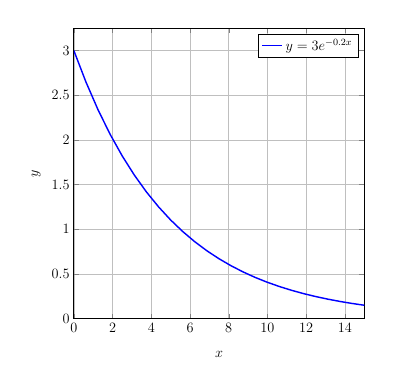
\begin{tikzpicture}[anchor = center, scale=.43]
			\begin{axis}[height=4in, width=4in,
				xmin=0,xmax=15,
				ymin=0,ymax=3.25,
				grid=major,
				%grid style={line width=.5pt, draw=gray!50},
				%major grid style={line width=.8pt,draw=gray!90},
				%axis lines=middle,
				%minor tick num=5,
				% enlargelimits=true,%{abs=0.5},
				axis line style={-latex, thick},
				ticklabel style={font=\large},
				ylabel = {$y$},
				xlabel = {$x$},
				% xlabel style={at={(ticklabel* cs:1)},anchor=north west},
				% ylabel style={at={(ticklabel* cs:1)},anchor=south west}
				x label style={at={(axis description cs:0.5,-0.1)},anchor=north,font=\large},
				y label style={at={(axis description cs:-0.1,.5)},rotate=0,anchor=south,font=\large},
				%         legend pos= north east, clip = true
				]
				\addplot+[no marks, very thick, blue,domain=0:15] { 3*exp(-0.2*x)};  \addlegendentry{\large $y = 3e^{-0.2x}$}
				% \only<4->{\addplot+[mark = +, thick,dashed, red] coordinates{ (10, 2.650) (30, 20.23) (70,53.55) (100,76.86) (130, 99.67)};  \addlegendentry{Lower 95\% confidence bound}}
			\end{axis}
		\end{tikzpicture}
		\pause
		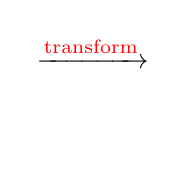
\begin{tikzpicture}[baseline={([yshift=-35pt]current bounding box.center)}]
			\node  at (0,5) {$\xrightarrow{\text{\rd transform}}$};
		\end{tikzpicture}
		\pause
		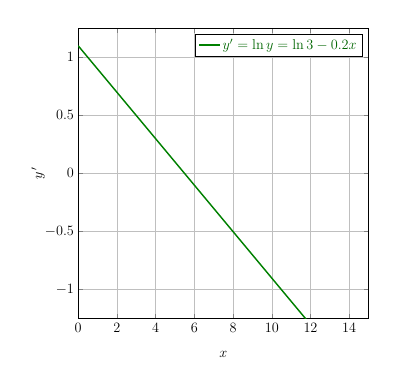
\begin{tikzpicture}[anchor= center,scale=.43]
			\begin{axis}[height=4in, width=4in,
				xmin=0,xmax=15,
				ymin=-1.25,ymax=1.25,
				grid=major,
				%grid style={line width=.5pt, draw=gray!50},
				%major grid style={line width=.8pt,draw=gray!90},
				% axis lines=middle,
				%minor tick num=5,
				% enlargelimits=true,%{abs=0.5},
				axis line style={-latex, thick},
				ticklabel style={font=\large},
				ylabel = {$y\, '$},
				xlabel = {$x$},
				% xlabel style={at={(ticklabel* cs:1)},anchor=north west},
				% ylabel style={at={(ticklabel* cs:1)},anchor=south west}
				x label style={at={(axis description cs:0.5,-0.1)},anchor=north,font=\large},
				y label style={at={(axis description cs:-0.1,.5)},rotate=0,anchor=south,font=\large},
				%          legend pos= north east, clip = true
				]
				% \coordinate (O) at (0,0);
				% \node[fill=white,circle,inner sep=0pt] (O-label) at ($(O)+(-135:10pt)$) {$O$};
				\only<4->{\addplot+[no marks, very thick, green!50!black,domain=0:15] {ln(3)  - 0.2*x};  \addlegendentry{\gr \large $y' = \ln y =  \ln 3 -0.2x$}}
			\end{axis}
		\end{tikzpicture}
	\end{exampleblock}
\end{frame}

\begin{frame}
	\frametitle{Transforming nonlinear models}
	
	\pause
	
	
	While a probabilistic model may not be linear in $x$, \pause its estimation is still considered a \textit{linear} regression \pause  if the model is
	\textbf{linear in the $\bm\beta_i$ parameters} after an appropriate data transformation.
	
	\bigskip
	
	\begin{block}{Intrinsically linear probabilistic model}
		A probabilistic model relating $Y$ to $x$ is \textbf{intrinsically linear} if, \pause
		by means of a transformation on $Y$ and/or $x$, \pause it can be reduced to a linear probabilistic model \pause $Y' = \beta_0  + \beta_1x' + \bm\epsilon'$.
	\end{block}
	
	\pause
	
	\medskip
	
	\begin{exampleblock}{Example 6: Probabilistic models of intrinsically linear functions}\pause
		\begin{enumerate}[<+->]
			\item $Y = \alpha e^{\beta x} \cdot \bm\epsilon$ \pause \quad (multiplicative exponential power model)
			\item $Y = \alpha x^{\beta} \cdot \bm\epsilon$ \pause \quad  (multiplicative power model)
			\item $Y = \alpha + \beta \log(x) +  \bm\epsilon$ \pause \quad (logarithmic model)
			\item $Y = \alpha + \beta \cdot \fr1x + \bm \epsilon$ \pause \quad (reciprocal model)
		\end{enumerate}
	\end{exampleblock}
\end{frame}

% \begin{frame}
	%   \frametitle{Parameter estimation}\pause 
	%   Parameter estimates can  computed via the \textbf{least-squares principle} as:
	
	%   \pause
	
	%   \begin{align}
		%     \hat\beta_1 & = \fr{\sum x'_i y'_i \pause - \fr1n\sum x'_i \sum y'_i}{\sum \lt(x'_i\rt)^2 \pause - \fr1n\lt(\sum x'_i \rt)^2} \\[2mm]
		%     \hat\beta_0 &= \fr{\sum y'_i - \hat\beta_1 \sum x'_i}{n} \pause = \ol y' \pause - \hat\beta_1 \ol{x}'
		%   \end{align}
	% \end{frame}

\begin{frame}
	\frametitle{Deciding when to transform data}\pause
	
	There are several diagnostic tools to determine how to proceed with choosing and estimating a suitable probabilistic model for a given dataset. \\ \pause
	
	\begin{enumerate}[<+->]
		\item The first step is to examine the data. At this stage, a linear or nonlinear relationship may be clear.
		\item Further, examine the residuals. The \textbf{standardized residuals} are commonly used. \pause This means that we subtract the mean (0) and divide by the standard deviation: \pause
		\begin{equation}
			\label{eq:51}
			e^*_i = \fr{y_i - \hat y_i}{s \sqrt{ 1 - \fr1n - \fr{(x_i - \ol x)^2}{S_{xx}}}} \quad i = 1, \ldots, n
		\end{equation}
		
		\pause
		The fundamental assumption of linear regression is that the variance in the data $\sigma^2$ is constant. \pause
		If a relationship is apparent, then a transformation of the data may be necessary.
		\begin{enumerate}
			\item A curved residual scatter plot indicates a nonlinear relationship
			\item A cone-shapped scatter plot indicates non-constant variance, in which case the \textbf{weighted least squares} approach must be used
		\end{enumerate}
		
	\end{enumerate}
\end{frame}

\begin{frame}
	\frametitle{Deciding when to transform data (cont.)}\pause
	
	
	\begin{enumerate}[<+->]\setcounter{enumi}{3}
		\item Create a normal probability plot (Q-Q plot) of the residuals to check that they are normally distributed (or examine the histogram). If not, then a transformation may be necessary.\pause
		
		\begin{figure}[h!]
			\centering
			\includegraphics[width = 0.3\textwidth]{qqplot_oldfaithful}
			\caption{Q-Q plot of standardized residuals for Old Faithful eruption durations regressed on the waiting times between eruptions}
			\label{fig:of}
		\end{figure}
		
		
		\item If abnormalities remain after the data are transformed, %(usually by taking logs of $y$ or $x$ or both),
		then more advanced techniques may be required (which are beyond the scope of this course).
	\end{enumerate}
\end{frame}


% \begin{frame}
	%   \frametitle{Deciding when to transform data (cont.)}\pause
	
	
	%   \begin{enumerate}[<+->]\setcounter{enumi}{4}
		
		%   \item If after the data are transformed (usually by taking logs of $y$ or $x$ or both), there are still abnormalities, then more advanced technqiues may be required (which are beyond the scope of this course).
		%   \end{enumerate}
	% \end{frame}



\section{Polynomial regression}

\begin{frame}
	\frametitle{Polynomial regression}\pause
	In some cases, a polynomial function provides a good approximation to the true regression function for a given dataset. \pause
	
	% \begin{onlyenv}<3->
		\begin{center}
			\visible<3->{\includegraphics[width=0.4\textwidth]{polyfit1}} \pause $\;$ \pause
			\visible<6->{\includegraphics[width=0.4\textwidth]{polyfit2}}
		\end{center}
		
		% \end{onlyenv}
	
	\pause
	
	% \begin{onlyenv}<5-10>
		\begin{block}{$k$-th degree polynomial regression model equation}\pause
			\begin{equation}
				\label{eq:20}
				Y = \beta_0 + \beta_1 x + \beta_2 x^2 + \cdots + \beta_k x^k + \bm \epsilon
			\end{equation}
			\pause
			where $\bm\epsilon$ is normally distributed: \pause $\mathcal{N}(0, \sigma^2)$
		\end{block}
		
		\pause
		
		This means that the expected value of $Y$ given $x$ can be written as:\pause
		\begin{equation}
			\label{eq:21}
			\mu_{Y \cdot x} = E(Y|X = x) = \beta_0 + \beta_1 x + \beta_2 x^2 + \cdots + \beta_k x^k
		\end{equation}
		% \end{onlyenv}
\end{frame}



\begin{frame}
	\frametitle{Polynomial regression and multiple regression}
	Polynomial regression can be considered a special case of multiple linear regression.\\ \pause
	
	For example, consider the model:
	\begin{equation*}
		Y = \beta_0 + \beta_1x + \beta_2 x^2 + \bm\epsilon
	\end{equation*}
	
	\pause
	
	If we set $x \to x_1$ and $x^2 \to x_2$, then the model becomes:\pause
	
	\begin{equation*}
		Y = \beta_0 + \beta_1x_1 + \beta_2x_2 +\bm\epsilon
	\end{equation*}
	\pause
	
	which can be taken as a multiple linear regression model with two predictor variables.
\end{frame}

\begin{frame}[fragile]
	\frametitle{Polynomial regression in practice}
	
	\begin{exampleblock}{Example 7: Effects of harvest date on yield of rice}\pause
		Data was collected on the date $x$ of harvesting (number of days after flowering) and yield $y$ (kg/ha) of rice. \pause
		The estimated parameters are:\pause
		\[\hat\beta_0 = -1070.4 \quad \hat\beta_1 = 293.48 \quad \hat\beta_2 = -4.5358 \] \pause
		Some of the computer program output reads: \pause
		\begin{verbatim}
			Predictor        Coef     Stdev     t-ratio       p
			Constant      -1070.4     617.3       -1.73   0.107
			DAYS           293.48     42.18        6.96   0.000
			DAYSSQD       -4.5358    0.6744       -6.73   0.000
			
			s = 203.9   R-sq = 79.4%   R-sq(adj) = 76.2%
		\end{verbatim}
	\end{exampleblock}
\end{frame}

\begin{frame}[fragile]
	\frametitle{Polynomial regression in practice}
	
	\begin{exampleblock}{Example 7: Effects of harvest date on yield of rice (cont.)}\pause
		\begin{enumerate}[(a)]
			\item Write the estimated regression function. \pause
			\begin{equation*}
				y = -1070.4 + 293.48x - 4.5358x^2
			\end{equation*}
			\pause
			
			\item Based on the computer output, which of the coefficients is a weak predictor? \pause
			Answer: the $p$-value of the intercept is 0.107, which means that at $\alpha = 0.05$ or even at $\alpha = 0.10$, we would fail to reject the null hypothesis that $\beta_0 = 0$.
		\end{enumerate}
	\end{exampleblock}
\end{frame}

\begin{frame}[fragile]
	\frametitle{Polynomial regression in practice}
	
	\begin{exampleblock}{Example 7: Effects of harvest date on yield of rice (cont.)}\pause
		\begin{enumerate}[(a)]\setcounter{enumi}{2}
			\item Sketch the regression line over the scatterplot of the data \pause
			\begin{tikzpicture}[scale=.5]
				\begin{axis}[height=4in, width=6in,
					xmin=15,xmax=50,
					ymin=2500,ymax=4000,
					grid=both,
					grid style={line width=.5pt, draw=gray!50},
					major grid style={line width=.8pt,draw=gray!90},
					axis lines=middle,
					minor tick num=5,
					enlargelimits={abs=0.5},
					axis line style={-latex, thick},
					ticklabel style={font=\large},
					ylabel = {Yield (kg/ha)},
					xlabel = {Days},
					% xlabel style={at={(ticklabel* cs:1)},anchor=north west},
					% ylabel style={at={(ticklabel* cs:1)},anchor=south west}
					x label style={at={(axis description cs:0.5,-0.1)},anchor=north,font=\large},
					y label style={at={(axis description cs:-0.1,.5)},rotate=90,anchor=south,font=\large},
					legend pos=outer north east
					]
					
					% \coordinate (O) at (0,0);
					% \node[fill=white,circle,inner sep=0pt] (O-label) at ($(O)+(-135:10pt)$) {$O$};
					\only<2->{\addplot+[mark = *, only marks] coordinates {(16,2508) (18,2518) (20, 3304) (22,3423) (24,3057) (26,3190) (28,3500) (30,3883)
							(32,3823) (34,3646) (36,3708) (38,3333) (40,3517) (42,3241) (44,3103) (46,2776)}; \addlegendentry{Sample data}}
					\only<3->{\addplot+[mark = +, very thick, red,domain=15:50] { -1070.4 + 293.48*x - 4.5358*x*x};  \addlegendentry{Regression line}}
					% \only<4->{\addplot+[mark = +, thick,dashed, red] coordinates{ (10, 2.650) (30, 20.23) (70,53.55) (100,76.86) (130, 99.67)};  \addlegendentry{Lower 95\% confidence bound}}
				\end{axis}
			\end{tikzpicture}
		\end{enumerate}
	\end{exampleblock}
\end{frame}

\begin{frame}
	\frametitle{Polynomial regression in MATLAB}
	
	\begin{exampleblock}{Example 8: Using the \texttt{polyfit} function}\pause
		Run the \texttt{polyfit\_example.m} script. Examine the results of the 2nd, 4th and 5th order polynomial regression estimates for the sample data.
		
		\begin{enumerate}[(a)]
			\item How can you improve the model estimate?
			\item Can you obtain the same results using the \texttt{fitlm} function?
		\end{enumerate}
	\end{exampleblock}
\end{frame}




\section{Logistic regression}

\begin{frame}
	\frametitle{Introduction to logistic regression}\pause
	If $y$ were a categorical variable, in the simplest case, $y \in \{0, 1\}$, \pause corresponding to success and failure. \\ \pause
	
	Rather than modeling $y$ directly, we need to model the \textit{probability} of $y$, i.e. $p = P(y=1)$ (success) or $P(y=0) = 1 - p$ (failure).
	
	\pause
	
	\begin{exampleblock}{Examples of categorical dependent variables}\pause
		\begin{itemize}[<+->]
			\item The probability that a car needs warranty service of a certain kind, which could depend on \textit{mileage}.
			\item The probability of avoiding a certain infection, which could depend on the \textit{dosage} in an inoculation.
			\item The probability in a certain year of not biking ($y = 0$), biking at least monthly ($y = 1$) or biking at least weekly ($y = 2$), which could very well depend on \textit{income}, \textit{preference}, \textit{safety} and \textit{car ownership}.
		\end{itemize}
	\end{exampleblock}
\end{frame}

\begin{frame}
	\frametitle{Logistic regression}\pause
	In this introduction, we will focus only on the binomial case, i.e. $y = 0$ or $y = 1$. \\ \pause
	
	\medskip
	
	We   denote $p(x)$ as the probability that $y = 1$ based on a given variable $x$. \\ \pause
	
	\medskip
	
	Since $ 0 \le p(x) \le 1$, we see that the linear model is no longer appropriate. \pause
	
	\medskip
	
	In logistic regression, the logistic function is used instead.\pause
	
	
	\begin{block}{Logistic function}\pause
		\begin{equation}
			\label{eq:40}
			p(x) = \fr{e^{\beta_0 + \beta_1 x}}{1 + e^{\beta_0 + \beta_1 x}}
		\end{equation}
	\end{block}
\end{frame}

\begin{frame}
	\frametitle{Logit function}
	For $\beta_1 > 0$, the logistic function increases w.r.t.\ $x$. \pause
	
	For $\beta_1 < 0$, the logistic function decreases w.r.t.\ $x$. \pause
	
	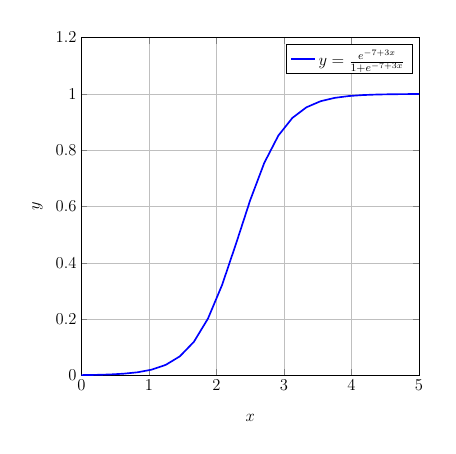
\begin{tikzpicture}[anchor = center, scale=.5]
		\begin{axis}[height=4in, width=4in,
			xmin=0,xmax=5,
			ymin=0,ymax=1.2,
			grid=major,
			% grid style={line width=.5pt, draw=gray!50},
			% major grid style={line width=.8pt,draw=gray!90},
			% axis lines=middle,
			% minor tick num=5,
			% enlargelimits=true,%{abs=0.5},
			axis line style={-latex, thick},
			ticklabel style={font=\large},
			ylabel = {$y$},
			xlabel = {$x$},
			% xlabel style={at={(ticklabel* cs:1)},anchor=north west},
			% ylabel style={at={(ticklabel* cs:1)},anchor=south west}
			x label style={at={(axis description cs:0.5,-0.1)},anchor=north,font=\large},
			y label style={at={(axis description cs:-0.1,.5)},rotate=0,anchor=south,font=\large},
			% legend pos= north east, clip = true
			]
			\addplot+[no marks, very thick, blue,domain=0:5] { exp(-7 + 3*x)/(1 + exp(-7 + 3*x)};  \addlegendentry{\large $y = \fr{e^{-7 + 3x}}{1 + e^{-7 + 3x}}$}
			% \only<4->{\addplot+[mark = +, thick,dashed, red] coordinates{ (10, 2.650) (30, 20.23) (70,53.55) (100,76.86) (130, 99.67)};  \addlegendentry{Lower 95\% confidence bound}}
		\end{axis}
	\end{tikzpicture}
	\pause \quad 
	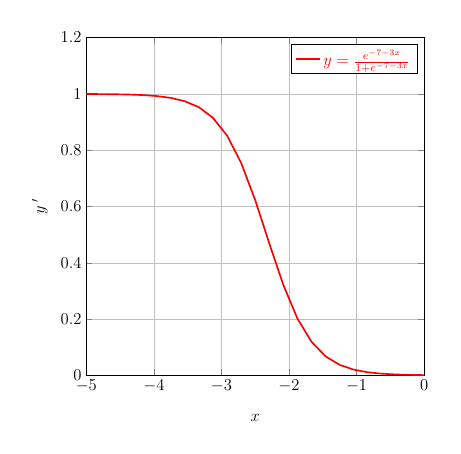
\begin{tikzpicture}[anchor= center,scale=.5]
		\begin{axis}[height=4in, width=4in,
			xmin=-5,xmax=0,
			ymin=0,ymax=1.2,
			grid=major,
			% grid style={line width=.5pt, draw=gray!50},
			% major grid style={line width=.8pt,draw=gray!90},
			% axis lines=middle,
			% minor tick num=5,
			% enlargelimits=true,%{abs=0.5},
			axis line style={-latex, thick},
			ticklabel style={font=\large},
			ylabel = {$y\, '$},
			xlabel = {$x$},
			% xlabel style={at={(ticklabel* cs:1)},anchor=north west},
			% ylabel style={at={(ticklabel* cs:1)},anchor=south west}
			x label style={at={(axis description cs:0.5,-0.1)},anchor=north,font=\large},
			y label style={at={(axis description cs:-0.1,.5)},rotate=0,anchor=south,font=\large},
			% legend pos= north east, clip = true
			]
			% \coordinate (O) at (0,0);
			% \node[fill=white,circle,inner sep=0pt] (O-label) at ($(O)+(-135:10pt)$) {$O$};
			\addplot+[no marks, very thick,red,domain=-5:0] {exp(-7 - 3*x)/(1 + exp(-7 - 3*x)};  \addlegendentry{\rd \large $y = \fr{e^{-7 - 3x}}{1 + e^{-7 - 3x}}$}
		\end{axis}
	\end{tikzpicture}
	
\end{frame}

\begin{frame}
	\frametitle{Odds ratio}\pause
	\textbf{Logistic regression} means that we assume $p(x)$ is related to $x$ as: \pause
	
	\begin{equation}
		\label{eq:52}
		\fr{p(x)}{1 - p(x)} = \pause e^{\beta_0 + \beta_1 x}
	\end{equation}
	\pause
	
	where the left-hand-side (LHS) is the \textit{odds ratio}. \pause
	
	
	\begin{block}{Odds ratio}\pause
		The odds ratio indicates how much more likely success is than failure. \pause
		
		\begin{equation}
			OR =  \fr{p(x)}{1  - p(x)} 
		\end{equation}
		
		\pause
		
		\textbf{Example:} If for a given value of $x$, the odds ratio is 3, then it means success is three times as likely as failure.
	\end{block}
\end{frame}

\begin{frame}
	\frametitle{Log odds}
	The logarithm of the odds ratio \pause (\textit{log odds}) is a linear function of the predictor $x$: \pause
	\begin{align*}
		\ln \lt( \fr{p(x)}{1  - p(x)}  \rt ) &= \ln  e^{\beta_0 + \beta_1 x} \\ \pause
		&= \beta_0 + \beta_1 x
	\end{align*}
	\pause
	
	The process of taking the log of the odds ratio is the \textbf{logit transformation}, \pause and $\ln\lt(\fr{p(x)}{1 - p(x)}\rt)$ is the 
	\textbf{logit function} ($logit(p)$). \pause
	
	\begin{itemize}
		\item This means that the parameter $\beta_1$ is the change in the log odds
		corresponding to a 1-unit increase in $x$. \pause
		
		\item   Consequently, the odds ratio itself changes by the multiplicative factor $e^{\beta_1}$ when $x$ increases by 1 unit.
	\end{itemize}
\end{frame}

\begin{frame}
	\frametitle{Logistic regression in practice}
	
	\begin{exampleblock}{Example 9: Probability of O-ring non-failure}\pause
		Data on launch temperature and incidence of [non-]failure for O-rings in 24 space shuttle launches prior to the \textit{Challenger} disaster of January 1986 were collected.\pause
		
		\begin{enumerate}[(a)]
			\item Run the MATLAB script \texttt{logistic\_regression\_example.m}. \pause
			\item What are the estimated parameters $\hat\beta_0$ and $\hat\beta_1$? \pause
			\textbf{Solution:} $\hat\beta_0 = -10.875$ \quad \pause $\hat\beta_1 = 0.1713$. \pause
			\item What is the change in the odds of success for each 1-degree increase in temperature?
		\end{enumerate}
	\end{exampleblock}
\end{frame}


\begin{frame}
	\frametitle{Parameter estimation in multiple regression}\pause
	We can write the true regression equation in matrix form as: \pause
	\begin{equation}
		\label{eq:6}
		\bm y = \bm X \bm \beta
	\end{equation}
	\pause where $\bm X$ is the $n \times k+1$ matrix:\pause
	\begin{equation}
		\label{eq:7}
		\bm X =
		\begin{bmatrix}
			1 & x_{11} & x_{12} & \cdots & x_{1k} \\
			1 & x_{21} & x_{22} & \cdots & x_{2k} \\
			\vdots & \vdots & \vdots &  \ddots & \vdots \\
			1 & x_{n1} & x_{n2} & \cdots & x_{nk} \\
		\end{bmatrix}
	\end{equation}
	\pause
	
	Using the least-squares principle, we can find the $SSE$ and take the partial derivatives with respect to the $\beta_i$'s and set these equations to zero to then solve for the $\hat\beta_i$'s.
\end{frame}

\begin{frame}
	\frametitle{Parameter estimation in multiple regression (cont.)}\pause
	This system  of \textbf{normal equations} can be written as:\pause
	\begin{equation}
		\label{eq:8}
		\bm{X^T X \hat\beta } = \bm{X^T y}
	\end{equation}\pause
	
	And thus:
	\begin{equation}
		\label{eq:9}
		\bm{\hat\beta} = \bm{\lt(X^T X\rt)^{-1}X^T y}
	\end{equation}
	
	We can then predict the $y$ value for a set of given values for $\bm x$ as:\pause
	\begin{equation}
		\label{eq:10}
		\hat y = \bm x^T  \bm{\hat\beta}
	\end{equation}
\end{frame}



% \section{Multiple regression}

% \begin{frame}
%   \frametitle{Multiple Regression}
%   If a dependent variable $y$  is related to two or more predictor variables, the estimation of linear model is called \textbf{multiple linear regression}:

%   \begin{block}{General additive multiple regression model equation}\pause
%     \begin{equation}
%       \label{eq:1}
%       Y = \beta_0 + \beta_1 x_1 + \beta_2 x_2 + \cdots + \beta_k x_k + \bm\epsilon
%     \end{equation}
%     \pause

%     where $k$ is the number of predictor variables.\\  \pause

%     The $\beta_i$'s are the \textbf{true regression coefficients} and are interpreted as the expected change in $Y$ associated with a 1-unit increase in $x_i$ while the other predictor variables are held fixed. 
%   \end{block}
% \end{frame}

% \begin{frame}
%   \frametitle{Multiple regression in practice}\pause
%   \begin{exampleblock}{Example 1: Ball bond shear strength}
%     An experiment was carried out to assess the impact of the variables $x_1 =$ force (gm), $x_2 =$ power (mW), $x_3 = $ temperature ($^\circ$C) and $x_4 = $ time (ms) on $y = $ ball bond shear strength (gm).
%     Based on the data collected, a statistical computer package gave the following least squares estimates:
%     \begin{equation*}
%       \hat\beta_0 = -37.48 \quad       \hat\beta_1 = 0.2117 \quad
%       \hat\beta_2 = 0.4983 \quad       \hat\beta_3 = 0.1297 \quad
%       \hat\beta_4 = 0.2583
%     \end{equation*}

%     \begin{enumerate}[(a)]
%     \item What is the average change in strength associated with a 1-degree increase in temperature when the other three predictors are held fixed?
%     \item What is the estimated regression equation?
%     \item What is the point prediction (point estimate of the mean value) of strength resulting from a force of 35 gm, power of 75 mW, temperature of 200$^\circ$C and a time of 20 ms?
%     \end{enumerate}
%   \end{exampleblock}
% \end{frame}

% \begin{frame}
%   \frametitle{Multiple regression in practice}\pause
%   \begin{exampleblock}{Example 1: Ball bond shear strength (cont.)}
%     \begin{enumerate}[(a)]\pause
%     \item The average change in strength associated with a 1-degree increase in temperature when the other three predictors are held fixed is \pause $\boxed{\gr 0.1297 \text{ gm}}$.\pause
%       \bigskip
      
%     \item The estimated regression equation is:\pause
%       \begin{equation*}
%         \hat y = -37.48 + 0.2117x_1 + 0.4983x_2 + 0.1297x_3 + 0.2583x_4
%       \end{equation*}
%     \pause

%   \item The point prediction of strength is given by:\pause
%     \begin{align*}
%       \hat y &= -37.48 + 0.2117(35) + 0.4983(75)  \\\pause
%              &\quad + 0.1297(200) + 0.2583(20) \\\pause
%              &= \boxed{\gr 38.41 \text{ gm}}
%     \end{align*}

%         \end{enumerate}

%   \end{exampleblock}
% \end{frame}



% \begin{frame}
%   \frametitle{$\bm{\hat\sigma}^2$ and $\bm R^2$}\pause

%   Recall the following terms: \pause
%   \begin{itemize}[<+->]
%   \item The \textbf{predicted} or \textbf{fitted values} $\hat y_i$ are obtained by substituting the predictor variables $x_i$ into the estimated regression equation.
%   \item The \textbf{residuals} are the differences between the observed and the predicted values: \pause $e_i = y_i - \hat y_i$
%   \item The closer the residuals are to zero, the better the estimate
%   \item A positive residual implies an under-estimate at that point
%   \item A negative residual implies an over-estimate at that point
%   \item The $SSE$ is the sum of squared errors/residuals
%   \end{itemize}
  
% \end{frame}


% \begin{frame}
%   \frametitle{$\bm{\hat\sigma}^2$ and $\bm R^2$ (cont.)}\pause
%   \begin{equation}
%     \label{eq:11}
%     SSE = \pause \sum (y_j - \hat y_j)^2 = \pause \sum\lt[ y_j -\lt(\hat\beta_0 + \hat\beta_1x_{1j} + \cdots + \hat\beta_k x_{kj}\rt)\rt]^2
%   \end{equation}
%   \pause

%   Since $k+1$ parameters are estimated, $k+1$ d.o.f.\ are lost. \pause  So, we can find the estimated variance as:\pause

%   \begin{equation}
%     \label{eq:12}
%     \hat\sigma^2 = \fr{SSE}{n - (k+1)} = MSE
%   \end{equation}
% \end{frame}

% \begin{frame}
%   \frametitle{$\bm{\hat\sigma}^2$ and $\bm R^2$ (cont.)}\pause
%   Recall that the $SST$ (measure of total variability in the data) is given by:
%   \pause

%   \begin{equation}
%     \label{eq:13}
%     SST = \sum(y_i - \ol{y})^2
%   \end{equation}

%   \pause

%   Thus, the proportion of total variation explained by the multiple regression model is: \pause
%   \begin{equation}
%     \label{eq:14}
%     R^2 = 1 - \fr{SSE}{SST}
%   \end{equation}

%   \pause

%   This is called the \textbf{coefficient of multiple determination}
% \end{frame}

% \begin{frame}
%   \frametitle{Adjusted $\bm R^2$}
%   While increasing the number of explanatory/predictor variables may improve the fit of the data to the model, there is a danger of \textbf{overfitting} whereby a higher $R^2$ may actually result from a worse model.

%   \pause

%   To balance the cost of using more parameters against the gain in $R^2$, we use the \textbf{adjusted coefficient of multiple determination} \pause (or simply, adjusted $R^2$):\pause

%   \begin{equation}
%     \label{eq:15}
%     R_a^2 = 1 - \fr{n-1}{n - (k+1)}\cdot\fr{SSE}{SST} = \fr{(n-1)R^2 - k}{n - 1 -k}
%   \end{equation}
% \end{frame}

% %https://towardsdatascience.com/overfitting-vs-underfitting-a-complete-example-d05dd7e19765
% \begin{frame}
%   \frametitle{Underfitting vs.\ overfitting}\pause

%   \textbf{Underfitting}: \pause high bias ($k = 1$) \pause

%   \includegraphics[width = .7\textwidth]{underfit}
% \end{frame}

% \begin{frame}
%   \frametitle{Underfitting vs.\ overfitting (cont.)}\pause

%   \textbf{Overfitting}: \pause low bias ($k = 25$) \pause

%   \includegraphics[width = .7\textwidth]{overfit}
% \end{frame}

% \begin{frame}
%   \frametitle{Underfitting vs.\ overfitting (cont.)}\pause

%   \textbf{Balanced fit}: \pause optimal bias-variance ratio ($k = 4$) \pause

%   \includegraphics[width = .7\textwidth]{balancedfit}
% \end{frame}


% \begin{frame}
%   \frametitle{Adjusted $\bm R^2$ in practice}\pause
%   The adjusted $R^2$ ($R_a^2$) adjusts the proportion of unexplained variation upward, thus: \pause
%   \begin{equation}
%     \label{eq:16}
%       R_a^2 < R^2
%   \end{equation}
%   \pause

%   \begin{exampleblock}{Example 2: Computing adjusted $R^2$} \pause
%     In a given regression model with $k = 2$, $R^2 = 0.66$ . With $k = 3$ (an additional explanatory variable), $R^2 = 0.70$. If $n = 10$, calculate the adjusted $R^2$ for each case.

%     \pause

%     For $k =2$: \pause
%     \begin{equation*}
%       R_a^2 = \fr{9(.66) - 2}{10 -3 } = 0.563 
%     \end{equation*}

%     \pause

%     For $k = 3$: \pause
%     \begin{equation*}
%       R_a^2 = \fr{9(.70) - 3}{10 -4 } = \pause 0.550
%     \end{equation*}
    
%   \end{exampleblock}
% \end{frame}

% \begin{frame}
%   \frametitle{ANOVA testing for multiple regression}\pause

%   In ANOVA for multiple regression, the null hypothesis is:\pause

%   \begin{equation}
%     \label{eq:17}
%     H_0: \beta_1 = \beta_2 = \cdots = \beta_k = 0
%   \end{equation}
%   \pause

%   The alternative hypothesis is: \pause \textit{at least one of the $\beta_i$'s is not zero $(i = 1,\ldots, k)$}.
% \end{frame}



 
%\begin{frame}[allowframebreaks]
%   \frametitle{References}
%   \AtNextBibliography{\scriptsize}
%   \setbeamertemplate{bibliography item}[text]
%   \printbibliography[heading=none]
  
% \end{frame}

%\printbibliography
\end{document}
%%% Local Variables:
%%% mode: latex
%%% TeX-master: t
%%% End:
